\chapter{ RAPPORT D’ÉTUDE : Refonte de la chaîne de traitement et de valorisation des données d’IPANEMA }
\minitoc
\label{chap2}
\newpage

%=====================================%
\section{Introduction}
\label{sec21}
%---------------------------------------------------------%
Le rapport d'action a présenté une synthèse du projet IPANEMA et de ses résultats. Ce rapport 
d'étude revient plus en détail sur la démarche suivie : l'analyse du besoin métier, le diagnostic 
de l'architecture existante, la formalisation des exigences, puis la conception de la nouvelle 
architecture Data et décisionnelle. 

%=====================================% 
\section{ Contexte et problématique}
\label{sec:sec22}
%=====================================% 
\subsection{ IPANEMA et la maîtrise des Tierces Parties }
IPANEMA, acronyme de International Partners Network & Management, est une solution 
informatique utilisée au sein de la R&D Dermo-Cosmétique & Personal Care (DC&PC) de 
Pierre Fabre pour accompagner le processus de maîtrise des Tierces Parties. Dans ce 
contexte, une Tierce Partie désigne une entité extérieure au groupe dont l’activité peut avoir 
un impact direct ou indirect sur la qualité d’un produit ou sur la sécurité du patient, du 
consommateur ou du client.

La collaboration avec ces acteurs implique donc un suivi permettant d’identifier et 
d’évaluer les risques associés à leurs activités. IPANEMA intervient comme support 
numérique de ce processus : l’application centralise les informations nécessaires à l’évaluation 
des Tierces Parties et permet aux différents acteurs concernés de participer à leur suivi.

Les informations collectées ne constituent cependant qu’une première étape. Pour 
qu’elles puissent réellement contribuer au pilotage de l’activité, elles doivent être transformées 
en informations fiables, compréhensibles et exploitables par les équipes Qualité. Le reporting 
occupe ainsi une place importante dans la chaîne de valeur d’IPANEMA : il constitue le point 
de rencontre entre les données produites par le processus d’évaluation et leur utilisation à des 
fins de suivi et de prise de décision.

Cette dimension est au cœur du projet présenté dans ce rapport. 

\begin{figure}[H]
    \centering
    \fbox{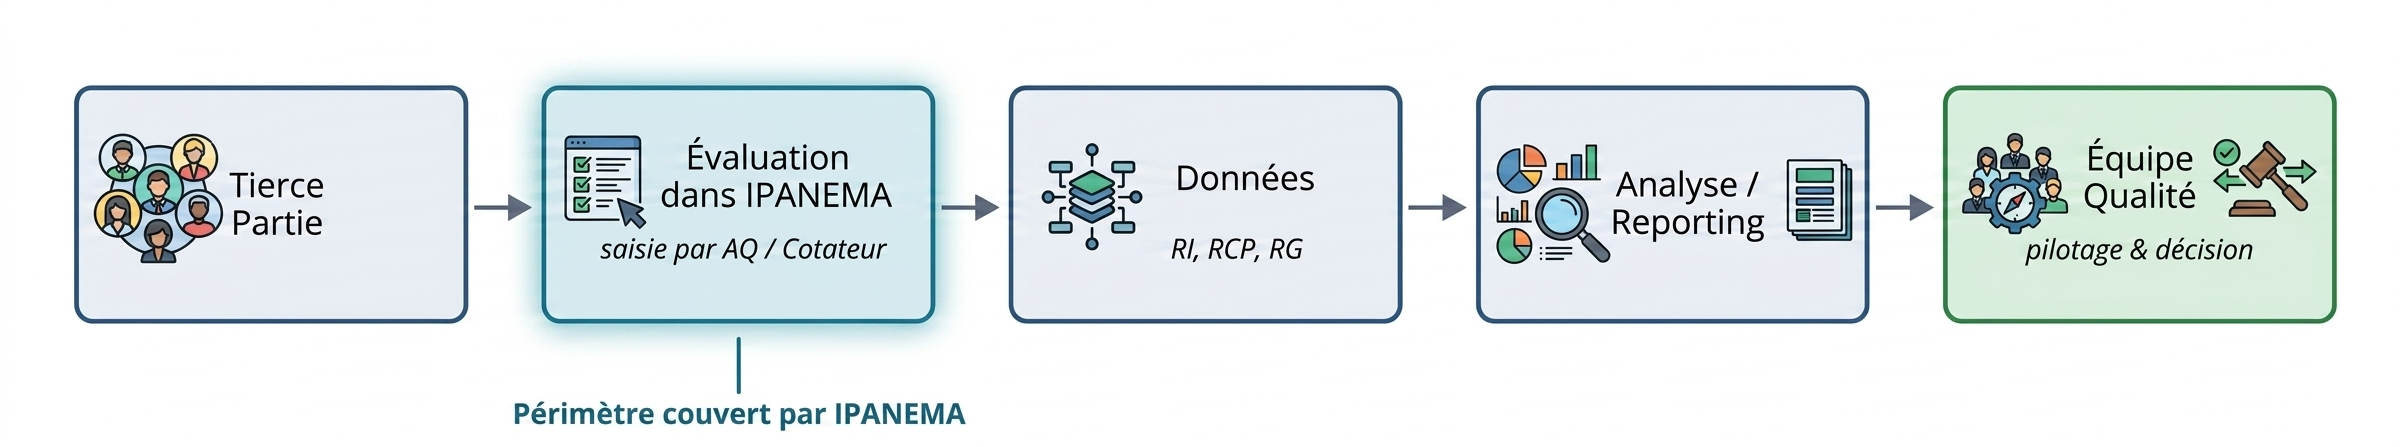
\includegraphics[width=5.5cm]{cover/figures/processusde_maîtrise_des_Tierces.jpg}}
    \caption{Positionnement d’IPANEMA dans le processus de maîtrise des Tierces Parties.}
    \label{fig:processusde_maîtrise_des_Tierces}
\end{figure}

%=====================================%    

\subsection{ Périmètre du projet IPANEMA V2  }\label{subsec:Perimètre du projet IPANEMA V2} 

Dans le cadre de son évolution, IPANEMA a fait l’objet d’une refonte vers une seconde 
version. Le projet global a été organisé autour de deux périmètres complémentaires. 

La Partie A concerne l’évolution de l’application métier développée sous Power Apps. 
Cette partie, confiée à un prestataire externe, comprend notamment la refonte des interfaces 
d’administration et de cotation, l’évolution de certaines fonctionnalités ainsi que la migration 
des données historiques. 

La Partie B concerne quant à elle la valorisation des données générées par IPANEMA. 
Elle comprend l’adaptation de la chaîne de traitement, l’intégration des calculs associés aux 
risques la mise à jour des indicateurs et la refonte du reporting. C’est sur ce second périmètre 
que s’inscrit mon projet d’alternance. 

Mon intervention ne s'est donc pas limitée à reproduire sous Power BI les visualisations 
historiquement disponibles sous Tableau. Les anomalies identifiées dans l'existant ont 
nécessité de réexaminer la manière dont les données étaient préparées, regroupées et mises 
en relation avant leur restitution. Le projet comporte ainsi deux dimensions étroitement liées : 
une dimension Data, portant sur la préparation, la structuration, la modélisation et la 
fiabilisation des données, et une dimension Business Intelligence, consacrée à la construction 
des indicateurs et à leur restitution dans un outil de pilotage adapté aux besoins des équipes 
Qualité. 

\begin{figure}[H]
    \centering
    \fbox{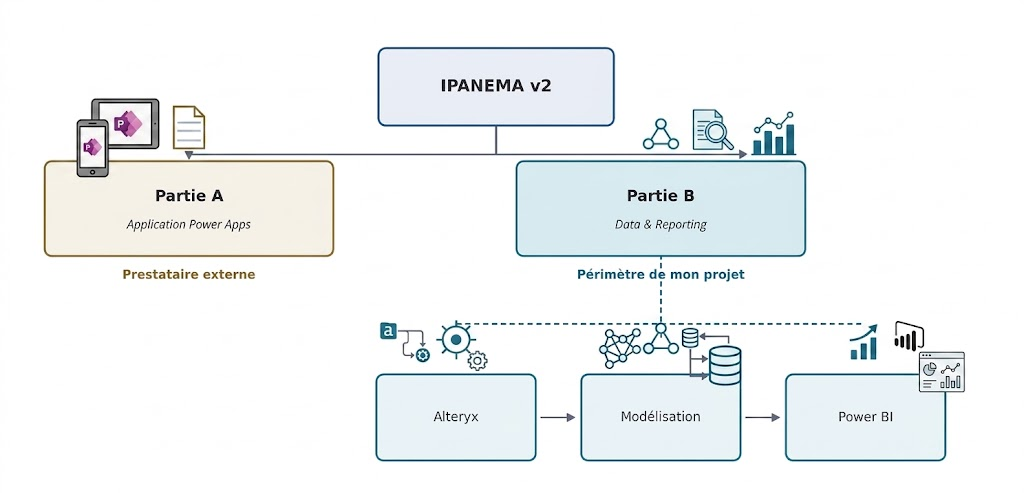
\includegraphics[width=5.5cm]{cover/figures/Périmètre_du_projet_IPANEMA_v2.jpg}}
    \caption{Périmètre du projet IPANEMA v2 : répartition entre la Partie A (application Power Apps, prestataire externe) et la Partie B (Data & Reporting, périmètre de mon projet).}
    \label{fig:Perimètre_du_projet_IPANEMA_v2}
\end{figure}


%=====================================%\n
\subsection{Problématique de l’étude}
%---------------------------------------------------------%
La première version du reporting IPANEMA reposait sur une chaîne associant Power Apps, SharePoint, Alteryx et Tableau. Les données saisies par les utilisateurs étaient stockées dans différentes listes SharePoint, puis consolidées au moyen de traitements Alteryx avant 
d’être restituées dans un dashboard Tableau. À l’usage, plusieurs limites ont été identifiées. La consolidation de données possédant 
des granularités différentes dans une table unique pouvait entraîner des duplications ou, selon 
les jointures réalisées, la disparition de certains enregistrements. Ces phénomènes étaient 
susceptibles d’affecter directement les indicateurs présentés aux utilisateurs. Des difficultés 
relatives à la maintenance, aux performances et à la lisibilité de la restitution ont également 
été remontées. 

Dans le même temps, l’environnement décisionnel du groupe évoluait progressivement 
vers l’écosystème Microsoft et Power BI. La migration constituait donc une opportunité pour 
ne pas simplement remplacer l’outil de visualisation, mais repenser plus globalement la chaîne 
de valorisation des données d’IPANEMA.

La problématique retenue pour cette étude est ainsi la suivante :

\textbf{Comment repenser la structuration et la restitution des données d’IPANEMA afin de fiabiliser le suivi des Tierces Parties, tout en proposant aux équipes Qualité un outil de pilotage performant, maintenable et intégré à l’écosystème Microsoft du groupe ?}
\\
La réponse à cette problématique nécessite d’abord de comprendre le processus métier 
à l’origine des données.

\section{Compréhension du besoin métier}

\subsection{Les acteurs et utilisateurs d’IPANEMA}

IPANEMA intervient dans un processus impliquant plusieurs catégories d’utilisateurs, 
dont les responsabilités et les besoins diffèrent. Quatre profils principaux sont identifiés dans 
l’application : \textbf{ Administrateur, Assurance Qualité (AQ), Cotateur et Consultation.}

L’\textbf{Administrateur} assure notamment la gestion des utilisateurs et de leurs droits d’accès. 
Son intervention garantit que chaque utilisateur dispose des fonctionnalités correspondant à 
son rôle. 

Le profil \textbf{Assurance Qualité} occupe une place centrale dans le processus. Il intervient 
dans le pilotage des Tierces Parties et des campagnes d’évaluation, dans la configuration de 
certains paramètres nécessaires à l’évaluation ainsi que dans la validation des informations 
renseignées. 

Le \textbf{Cotateur} appartient aux équipes métier en relation avec la Tierce Partie. Il intervient 
directement dans le processus d’évaluation en renseignant les critères qui relèvent de son 
périmètre. 

Enfin, le profil \text{Consultation} dispose d’un accès en lecture aux informations et 
évaluations finalisées, sans possibilité de modification. 

Cette diversité de profils implique que les données produites par IPANEMA ne répondent 
pas uniquement à une logique de stockage. Elles représentent le résultat d’un processus 
collaboratif, au cours duquel plusieurs acteurs interviennent successivement sur une même évaluation. Cette caractéristique aura une incidence directe sur la manière dont les données 
devront être modélisées, comme le montre la partie suivante.

\begin{figure}[H]
    \centering
    \fbox{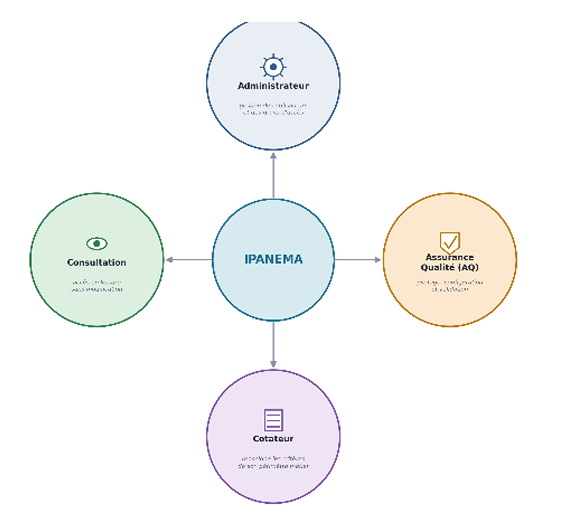
\includegraphics[width=0.25\textwidth]{cover/figures/quatre_profils_d'utilisateurs.png}}
    \caption{Les quatre profils d'utilisateurs d'IPANEMA et leur rôle dans le processus d'évaluation des Tierces Parties.}
    \label{fig:quatre_profils_d'utilisateurs}
\end{figure}


\subsection{Processus d’évaluation d’une Tierce Partie }

L’évaluation d’une Tierce Partie est réalisée dans le cadre d’une campagne. Une grille 
d’évaluation est générée, puis renseignée successivement par les acteurs concernés. 

Le Cotateur commence par compléter les critères correspondant à son périmètre 
métier. Une fois cette étape terminée, l’évaluation est transmise à l’Assurance Qualité, qui 
complète à son tour les éléments relevant de son domaine de responsabilité. L’AQ peut 
ensuite valider l’évaluation ou la retourner au Cotateur lorsqu’une correction ou un 
complément est nécessaire. Les changements de statut permettent ainsi de suivre la 
progression de l’évaluation jusqu’à sa finalisation.  

Ce fonctionnement est important d’un point de vue Data. Une Tierce Partie peut être 
associée à plusieurs campagnes et plusieurs évaluations au cours du temps. Une évaluation 
comporte elle-même plusieurs critères. Ces différents niveaux d’information ne possèdent 
donc pas nécessairement la même granularité : une donnée décrivant une Tierce Partie n’a 
pas le même niveau de détail qu’une donnée décrivant une campagne, une évaluation ou un 
critère. Leur rapprochement doit donc respecter les relations qui existent entre ces objets 
métier. Cette notion constitue l'un des points structurants du projet, et sera au cœur du 
diagnostic présenté en 2.3. 

\begin{figure}[H]
    \centering
    \fbox{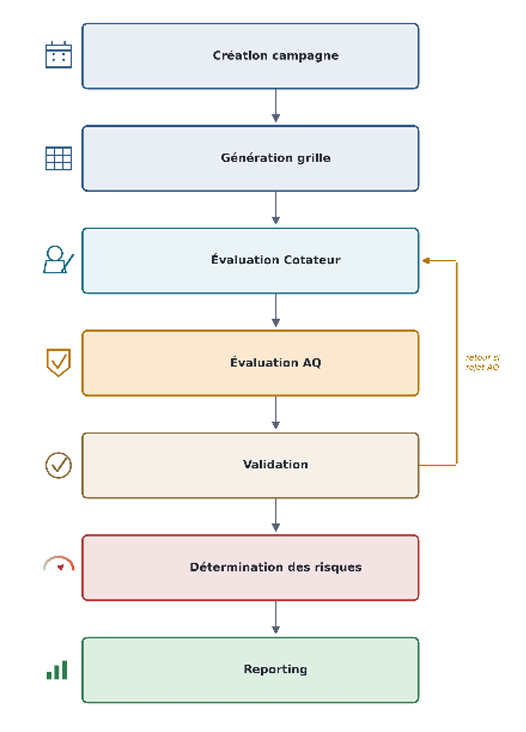
\includegraphics[width=0.25\textwidth]{cover/figures/processus_evaluation_tierce_partie.png}}
    \caption{Processus d'évaluation d'une Tierce Partie, de la création de la campagne au reporting. }
    \label{processus_evaluation_tierce_partie}
\end{figure}

\subsection{Les niveaux de risque}

Le processus d'évaluation repose sur trois notions de risque, dont le calcul constitue l'une 
des évolutions attendues de la solution cible : \textbf{le Risque Intrinsèque (RI), le Risque Conformité et Performance (RCP), et le Risque Global (RG)} qui en résulte.
\textbf{Le Risque Intrinsèque} caractérise le profil de risque propre à une Tierce Partie, 
indépendamment de la qualité de son exécution. Il est évalué annuellement par un utilisateur 
du profil AQ, à partir de sept critères portant sur des caractéristiques structurelles de la Tierce 
Partie : sa criticité, son niveau d'expertise et de savoir-faire, la complexité de la prestation (y 
compris en cas de sous-traitance en cascade), le référentiel qualité opposable, sa certification 
qualité et le volume de prestations attendu. Chaque critère est noté selon le niveau constaté, 
puis pondéré par un facteur qui varie selon que la Tierce Partie relève ou non du statut CDMO 
(\textbf{C}ontract \textbf{D}evelopment and \textbf{M}anufacturing \textbf{O}rganization). La somme des scores obtenus est 
ensuite comparée à la somme des scores maximum théoriquement atteignables, ce qui 
permet de classer le RI selon trois niveaux : LOW, MEDIUM, HIGH au moyen de seuils 
exprimés en fraction du score maximum.\\

\textbf{Le Risque Conformité et Performance} évalue, quant à lui, la manière dont la Tierce 
Partie exécute effectivement ses prestations. Il combine deux volets évalués par des profils 
distincts : un volet "Qualité", renseigné par l'AQ à partir des résultats d'audit et de la conformité 
qualité de la prestation, et un volet "Métier", renseigné par le Cotateur à partir de critères 
opérationnels tels que la qualité des livrables, la traçabilité, le respect des délais, le relationnel, 
les compétences techniques et la capacité d'innovation. Le score global obtenu est classé 
selon la même logique de seuils que pour le RI. Une particularité du RCP est qu'il n'est calculé 
que lorsque l'ensemble des évaluations de la Tierce Partie sur la campagne sont clôturées ; 
lorsqu'une Tierce Partie fait l'objet de plusieurs évaluations, le RCP retenu correspond à leur 
moyenne — une règle qui a une incidence directe sur la conception de la chaîne de données, 
puisqu'elle impose de disposer, avant le calcul, du statut de clôture de chaque évaluation 
associée.\\

\textbf{Le Risque Global} ne résulte pas d'une moyenne entre RI et RCP, mais d'une 
combinaison matricielle des deux niveaux. Cette logique traduit une approche volontairement 
conservatrice : une Tierce Partie présentant un RI élevé conserve un RG élevé même si son 
RCP est satisfaisant, ce qui reflète le fait que le risque intrinsèque (lié à la nature même de 
l'activité sous-traitée) ne peut être compensé par une bonne performance d'exécution. 
\\
Cette architecture de calcul, à trois niveaux imbriqués, a directement structuré la 
conception du modèle de données : elle impose de conserver la traçabilité des critères, des 
notes et des pondérations par campagne (ces paramètres pouvant évoluer d'une campagne 
à l'autre) et de restituer non seulement le RG final mais aussi les niveaux intermédiaires RI et 
RCP qui le composent. C'est précisément cette exigence d'historisation et de granularité qui 
rendait la logique de table unique inadaptée, comme le montre le diagnostic qui suit. 

\section{Analyse de l’existant et diagnostic}
\subsection{Architecture initiale}
Avant la refonte, les informations utilisées par IPANEMA provenaient principalement des 
deux applications Power Apps IPANEMA-Admin et IPANEMA-Cotation. Les données saisies 
étaient réparties dans 19 listes SharePoint.\\

Ces listes constituaient les différentes sources nécessaires à la restitution. Des workflows 
Alteryx permettaient de récupérer et de transformer les informations issues de SharePoint, 
auxquelles venaient également s’ajouter certaines données provenant de Trackwise. Les 
différentes sources étaient ensuite rapprochées afin de construire une table finale unique 
utilisée par Tableau.  

L’architecture pouvait ainsi être représentée de la manière suivante : 

\begin{center}
\begin{tcolorbox}[
    colframe=gray!60,       % Bordure gris doux
    colback=gray!4!white,   % Fond très clair
    boxrule=0.8pt,          % Épaisseur du cadre
    arc=5pt,                % Coins légèrement arrondis
    width=\textwidth,       % S'adapte à la largeur du texte
    halign=center,          % Centrage parfait du contenu
    top=8pt, bottom=8pt
]
\small\bfseries
Power Apps 
\;\textcolor{gray!80}{$\longrightarrow$}\; 
19 listes SharePoint 
\;\textcolor{gray!80}{$\longrightarrow$}\; 
Alteryx 
\;\textcolor{gray!80}{$\longrightarrow$}\; 
Table à plat 
\;\textcolor{gray!80}{$\longrightarrow$}\; 
Tableau
\end{tcolorbox}
\end{center}

Cette architecture avait l’avantage de fournir à l’outil de restitution un jeu de données 
directement exploitable. Cependant, la concentration de données de natures et de 
granularités différentes dans une même table a progressivement montré ses limites. 

\begin{figure}[H]
    \centering
    \fbox{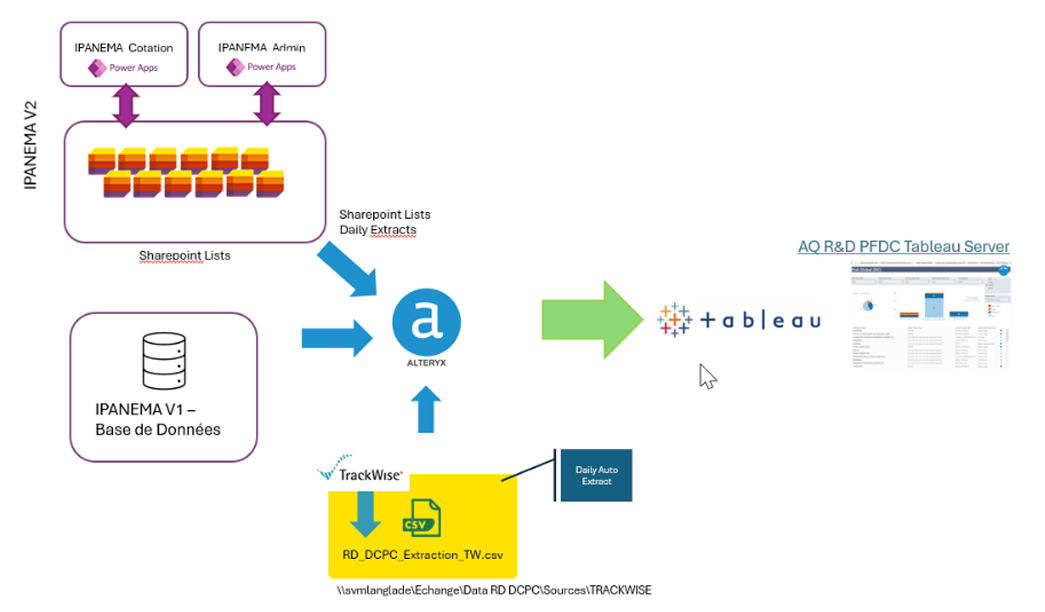
\includegraphics[width=0.25\textwidth]{cover/figures/Architecture_initiale_d'IPANEMA.png}}
    \caption{Architecture initiale d'IPANEMA : des sources de données jusqu'à la restitution de l'équipe Qualité (AQ R&D DCPC).}
    \label{Architecture_initiale_d'IPANEMA}
\end{figure}

\subsection{Analyse du traitement initial }
Le rôle d'Alteryx dans l'architecture initiale consistait à assurer les opérations d'extraction, 
de transformation et de préparation nécessaires avant la restitution des données. La difficulté 
ne résidait cependant pas dans l'utilisation d'Alteryx en elle-même, mais dans la logique de 
consolidation retenue : les informations issues des différentes sources étaient 
progressivement rapprochées au moyen de jointures successives, chaque nouvelle liste 
SharePoint étant intégrée à la table en cours de construction. Le schéma suivant illustre ce 
principe de manière simplifiée.  

\begin{figure}[H]
    \centering
    \fbox{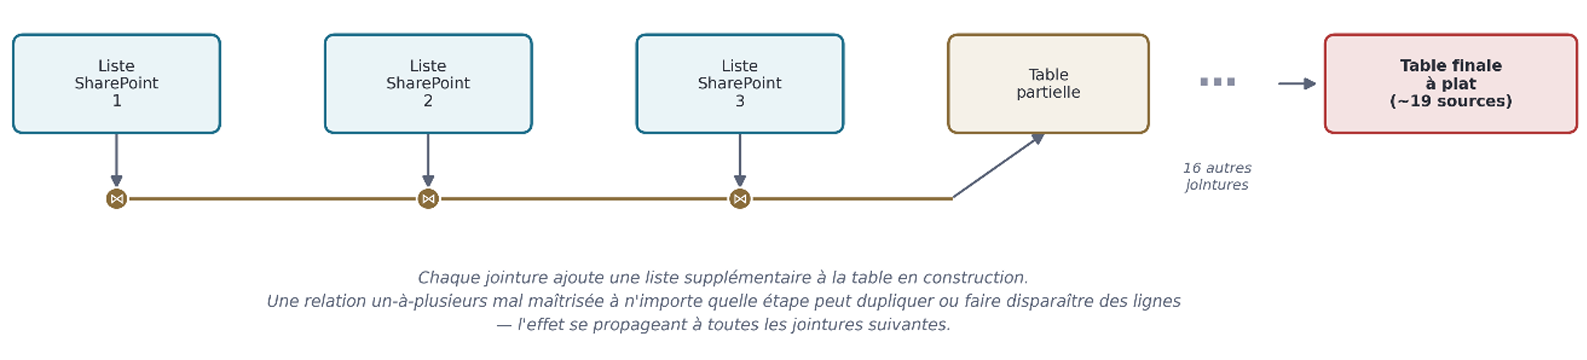
\includegraphics[width=0.25\textwidth]{cover/figures/jointures_successives_des_listes.png}}
    \caption{Principe de construction de l'ancienne table à plat : jointures successives des listes SharePoint en cascade.}
    \label{jointures_successives_des_listes}
\end{figure}

Ce principe, bien que simple dans sa logique, se traduisait dans la pratique par un 
enchaînement d'une vingtaine de jointures successives, correspondant chacune à l'intégration 
d'une nouvelle liste SharePoint. Le workflow réel, nettement plus dense que sa représentation 
schématique, donne une idée concrète de la complexité opérationnelle qui en résultait — 
complexité qui constitue en elle-même l'un des facteurs à l'origine des limites identifiées plus 
loin dans ce chapitre.

\begin{figure}[H]
    \centering
    \fbox{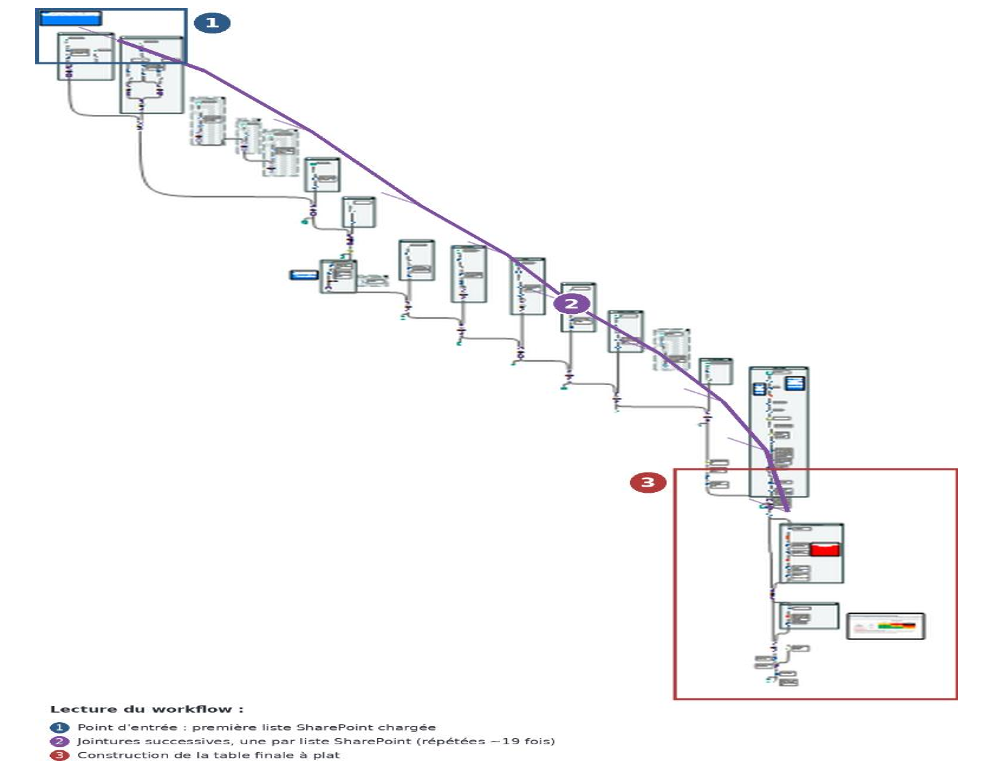
\includegraphics[width=0.25\textwidth]{cover/figures/Ancien_workflow_alteryx.png}}
    \caption{Ancien workflow Alteryx.}
    \label{Ancien_workflow_alteryx}
\end{figure}

Cette densité illustre un premier constat : au-delà des anomalies ponctuelles qu'elle a 
pu produire, cette architecture représentait déjà, par sa seule structure, un défi de 
maintenabilité. Mais la conséquence la plus directe de cette logique de jointures en cascade 
concerne la donnée elle-même. Les objets métier manipulés n'étaient en effet pas tous définis 
au même niveau de détail : une Tierce Partie peut, par exemple, être associée à plusieurs 
évaluations. Si les informations décrivant la Tierce Partie sont fusionnées directement avec 
celles décrivant chacune de ses évaluations, les données de la Tierce Partie sont 
nécessairement répétées pour chaque évaluation correspondante. Cette répétition n'est pas 
problématique en elle-même, elle le devient lorsque la table résultante est utilisée pour 
effectuer des comptages ou des agrégations sans tenir compte de cette granularité. \\

Cette architecture en cascade a ainsi une conséquence structurelle importante : une 
relation un-à-plusieurs mal maîtrisée à n'importe quelle étape de l'enchaînement se propage 
à l'ensemble des jointures suivantes, amplifiant mécaniquement le risque de duplication ou de 
perte d'enregistrements à mesure que le nombre de sources intégrées augmente. C'est 
précisément ce phénomène qui est détaillé dans le diagnostic ci-après. 

\subsection{Limites et anomalies identifiées}

L’analyse de l’existant, menée notamment lors des échanges avec le développeur du 
dashboard Tableau, mon maître d’apprentissage et les équipes Qualité, a permis de mettre 
en évidence plusieurs catégories de limites.

\textbf{a) Duplication des données}\\
La première difficulté concernait la duplication de certains enregistrements. Lorsqu’une 
relation de type un-à-plusieurs était intégrée dans la table unique, une même information 
pouvait être répétée sur plusieurs lignes. \\
Ces duplications pouvaient avoir une incidence directe sur certains indicateurs. Un 
comptage réalisé sans tenir compte de la granularité réelle des données risquait alors de 
comptabiliser plusieurs fois un même objet métier.

\text{b) Disparition de certains enregistrements}\\
Le phénomène inverse pouvait également se produire. Selon le type de jointure et la 
disponibilité des clés utilisées pour rapprocher les sources, certains enregistrements pouvaient 
ne pas être conservés dans le jeu de données final. \\
Une Tierce Partie présente dans une source pouvait ainsi ne plus apparaître dans le 
dashboard lorsque les conditions nécessaires à son rapprochement avec une autre table 
n’étaient pas satisfaites. 

\textbf{c) Valeurs manquantes interprétées à tort comme des notes. }\\
Ce point constitue l'une des anomalies les plus critiques identifiées, car elle ne produisait 
pas une simple erreur visible, mais une fausse donnée silencieuse : un résultat en apparence 
cohérent, mais construit sur une base erronée. Le mécanisme se déroule en plusieurs étapes. 
D'abord, comme détaillé en 2.3.2, la logique de jointures en cascade pouvait dupliquer certains 
enregistrements lorsqu'une relation un-à-plusieurs était mal maîtrisée. Parmi ces lignes 
dupliquées, certaines correspondaient à des critères ou des évaluations pour lesquels aucune 
note n'avait réellement été attribuée par l'utilisateur : l'évaluation était simplement absente, 
non renseignée. Le traitement existant, plutôt que de conserver cette absence de valeur telle 
quelle, la remplaçait automatiquement par 0. \\
C'est à ce stade que le problème devient critique : dans la logique de notation du RI et 
du RCP (cf. 2.2.3), 0 n'est pas une valeur neutre mais c'est la meilleure note possible, celle 
correspondant au niveau de risque le plus favorable. Une case vide, remplie automatiquement 
par 0, n'était donc pas traitée comme "pas d'information disponible", mais comme "cette Tierce 
Partie a été évaluée, et elle a obtenu la meilleure note sur ce critère". Une Tierce Partie qui 
n'avait tout simplement pas été évaluée sur un critère donné se retrouvait ainsi, après 
traitement, avec un score identique à celui d'une Tierce Partie réellement évaluée et jugée 
sans aucun risque sur ce critère. Le système ne pouvait plus distinguer ces deux situations 
pourtant radicalement différentes « on ne sait pas » et « on sait, et c'est excellent » produisant 
exactement le même résultat chiffré. Cette confusion faussait mécaniquement à la baisse les 
scores globaux RI et RCP des Tierces Parties concernées, pouvant les faire apparaître comme 
moins risquées qu'elles ne l'étaient réellement, un biais d'autant plus dangereux qu'il restait 
invisible sans investigation approfondie. \\

À cette confusion s'ajoutaient deux anomalies connexes, également liées au traitement 
des données absentes : certaines valeurs N/A remontaient dans certains cas jusque dans la 
restitution finale, sans traitement en amont, et certains enregistrements comportaient dans les 
données sources la valeur texte littérale "Null" plutôt qu'une valeur réellement vide : une 
nuance que les traitements existants ne géraient pas correctement, ce qui pouvait à son tour 
entraîner des duplications de lignes lors des jointures. Ce dernier cas a par exemple été 
identifié sur des partenaires dont l'activité est de type Development et le statut CDMO. 

\textbf{d) Complexité des calculs }\\
La restitution des risques RI, RCP et RG nécessite l’application de règles métier 
spécifiques. La structure de la table finale rendait certains traitements difficiles à maintenir et 
pouvait conduire à des résultats ne correspondant pas systématiquement aux valeurs 
attendues. 

\textbf{e) Maintenabilité }\\
La concentration d’une grande quantité d’informations dans une table unique augmentait 
également la complexité de maintenance. Toute évolution d’une source, d’une règle métier ou 
d’un indicateur pouvait nécessiter d’intervenir sur une chaîne de transformations comportant 
de nombreuses dépendances.\\

\textbf{Exemple concret} \\
L'écart observé sur l'indicateur de satisfaction "Innovation" du partenaire Cebiphar 
(campagne 2025) illustre concrètement l'impact de cette confusion entre absence d'évaluation 
et note favorable. Le dashboard Tableau affichait pour ce critère une valeur de 0,39, nettement 
inférieure aux autres critères de la même Tierce Partie, pourtant tous évalués de manière 
cohérente et satisfaisante. 

\begin{figure}[H]
    \centering
    \fbox{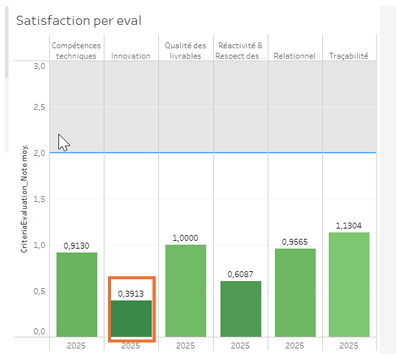
\includegraphics[width=0.1\textwidth]{cover/figures/valeur_anormalement_basse.png}}
    \caption{Ancien dashboard Tableau : satisfaction par critère pour Cebiphar (campagne 2025), avec une valeur anormalement basse sur le critère Innovation (0,39).}
    \label{valeur_anormalement_basse}
\end{figure}

L'analyse de cet écart a montré que le calcul Tableau intégrait, dans la moyenne du 
critère, les évaluations au statut "Not Evaluated", c'est-à-dire des évaluations non réalisées au 
même titre que les évaluations réellement renseignées. Cette confusion, décrite plus haut, 
faussait mécaniquement l'indicateur à la baisse.

Le nouveau dashboard Power BI, qui exclut correctement les statuts "Not Evaluated" du 
calcul, restitue pour ce même critère une valeur de 1,00 soit la note maximale, cohérente avec 
les autres critères de ce partenaire. 

\begin{figure}[H]
    \centering
    \fbox{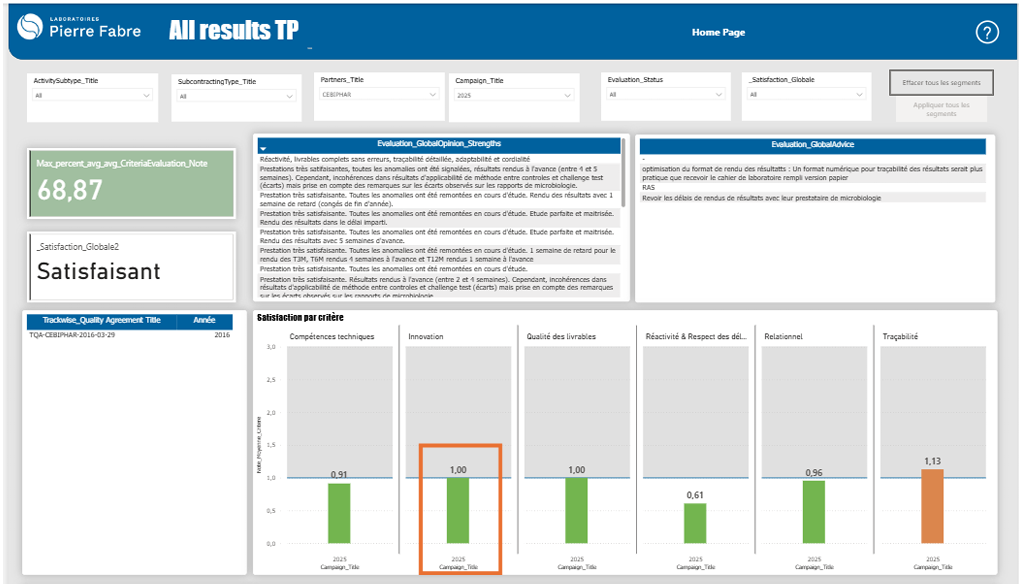
\includegraphics[width=0.1\textwidth]{cover/figures/Nouveau_dashboard_Power_BI.png}}
    \caption{Nouveau dashboard Power BI : satisfaction par critère pour Cebiphar (campagne 2025), avec une valeur corrigée de 1,00 sur le critère Innovation.}
    \label{Nouveau_dashboard_Power_BI}
\end{figure}

Cette correction a été vérifiée directement à la source, dans la liste SharePoint 
CriteriaEvaluation. En filtrant les évaluations sur le critère Innovation et en excluant les statuts 
"Not Evaluated", l'ensemble des notes réellement attribuées par les utilisateurs affiche une 
valeur de 1, confirmant que la valeur de 0,39 observée dans Tableau ne provenait pas d'une 
évaluation défavorable, mais bien de l'inclusion erronée d'évaluations non renseignées dans 
le calcul de la moyenne.

\begin{figure}[H]
    \centering
    \fbox{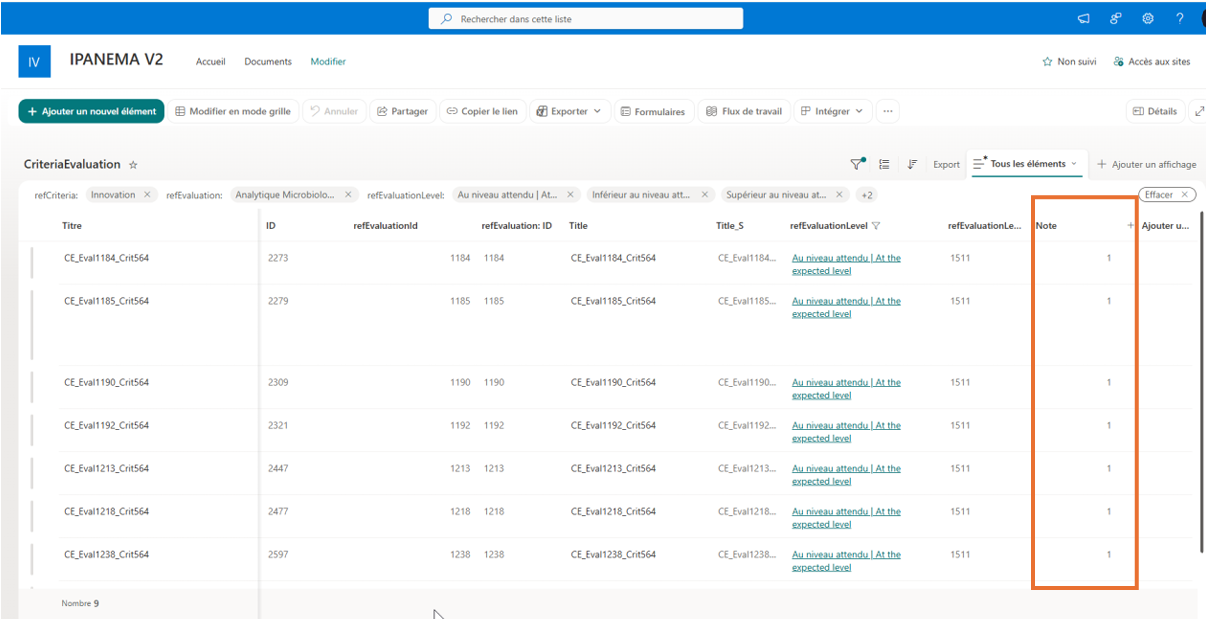
\includegraphics[width=0.1\textwidth]{cover/figures/Extrait_de_la_liste_SharePoint_CriteriaEvaluation.png}}
    \caption{Extrait de la liste SharePoint CriteriaEvaluation, filtré sur le critère Innovation : les notes effectivement attribuées valent toutes 1, confirmant la valeur restituée par Power BI.}
    \label{Extrait_de_la_liste_SharePoint_CriteriaEvaluation}
\end{figure}

La vérification à la source a par ailleurs révélé une difficulté supplémentaire : la colonne 
refEvaluationLevel de la table CriteriaEvaluation, censée permettre de distinguer les critères 
évalués des critères non évalués, comportait en réalité deux variantes distinctes du libellé "non 
évalué" (une différence de casse dans la traduction anglaise du libellé). Un filtre appliqué sur 
une seule de ces deux valeurs aurait donc laissé passer une partie des critères non évalués, 
faussant à nouveau le résultat. La vérification présentée en figure 11 a été réalisée en excluant 
systématiquement les deux variantes, afin de ne conserver que les critères réellement évalués 
illustrant, à une échelle plus fine encore, la même exigence de rigueur sur le traitement des 
données manquantes que celle décrite au point c).\\
Ce cas démontre, sur un exemple réel et vérifié à la source, la nécessité identifiée en 
amont : distinguer explicitement l'absence d'évaluation d'une évaluation réellement favorable, 
faute de quoi les indicateurs de risque et de performance perdent leur fiabilité avec un écart 
pouvant dépasser 0,6 point sur une échelle de 0 à 1, comme observé ici.

\subsection{Diagnostic}
L'analyse menée montre que les limites observées ne peuvent pas être attribuées à l'outil 
de visualisation seul : le dashboard Tableau restituait fidèlement les données qu'on lui 
transmettait, la défaillance se situant en amont, dans leur préparation.
\\
Trois causes s'en dégagent. Une cause architecturale : les jointures en cascade 
consolidaient des objets métier de granularités différentes dans une table unique, propice aux 
duplications et aux pertes d'enregistrements. Une cause sémantique : la confusion entre 
absence d'évaluation et note de 0 conduisait le système à traiter deux réalités opposées 
comme une seule donnée. Une cause liée à la gouvernance du référentiel : l'incohérence des 
valeurs de référence, comme le double libellé "non évalué", pouvait fausser les traitements en 
aval même lorsque leur logique était correcte.
\\
Le passage à Power BI ne pouvait donc pas se limiter à une migration à l'identique du 
dashboard existant : cela aurait déplacé l'interface de restitution sans corriger aucune de ces 
causes. La refonte devait intervenir à plusieurs niveaux : la préparation des données, pour 
limiter les effets en cascade des jointures ; la gestion explicite des valeurs manquantes ; 
l'organisation des données en entités cohérentes respectant leur granularité ; les relations 
entre ces entités, reconstruites au niveau du modèle plutôt qu'à plat ; le calcul des indicateurs 
RI, RCP et RG ; et leur restitution aux utilisateurs.
\\
Ce diagnostic constitue le point de départ de la solution proposée et structure la formalisation des exigences qui suit. 

\section{Formalisation du besoin et des exigences}
\subsection{Expression du besoin : Diagramme « bête à cornes »}
Afin de formaliser la finalité du projet indépendamment des choix technologiques, le 
besoin a été représenté à l’aide du diagramme « bête à cornes ». \\
Il permet de répondre à trois questions fondamentales : \\
\textbf{À qui le système rend-il service ?}
Aux équipes Qualité de la R&D DC&PC chargées du suivi des Tierces Parties. \\
\textbf{Sur quoi agit-il ?}
Sur les données issues de l’évaluation et du suivi des Tierces Parties. \\
\textbf{Dans quel but ? }
Fournir une information fiable et exploitable permettant de faciliter leur pilotage et la maîtrise 
des risques associés.

\begin{figure}[H]
    \centering
    \fbox{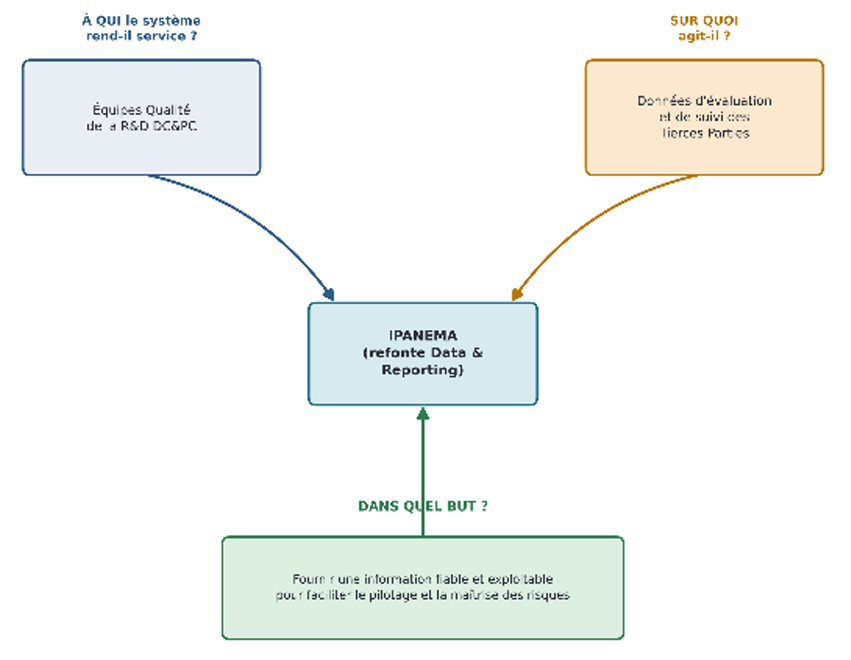
\includegraphics[width=0.1\textwidth]{cover/figures/Formalisation_du_besoin_du_projet_IPANEMA.png}}
    \caption{Formalisation du besoin du projet IPANEMA selon la méthode « bête à cornes »}
    \label{Formalisation_du_besoin_du_projet_IPANEMA}
\end{figure}

L’intérêt de cette représentation est de rappeler que la finalité du projet n’est pas la 
migration vers Power BI en elle-même. La technologie constitue un moyen permettant de 
répondre à un besoin métier : mettre à disposition des équipes Qualité une information fiable 
leur permettant de piloter les Tierces Parties.

\subsection{Besoins exprimés par les utilisateurs} 
Les attentes des équipes Qualité se sont précisées progressivement, au fil des 
réunions d'avancement et des retours sur les versions successives du dashboard. Six 
grandes catégories de besoins se dégagent, chacune distinguant ce qui a été exprimé par 
les utilisateurs de sa traduction technique.


%=====================================%
\section{Campagne de tests du premier module de la plateforme} 
%---------------------------------------------------------%

Dans la continuité de la phase de développement, une campagne de tests a été menée afin de valider la première version du module de recrutement des bénéficiaires de la plateforme RI2S. Cette étape avait pour objectif de garantir la conformité fonctionnelle et technique des premières fonctionnalités livrées, et d’évaluer la robustesse de la solution en vue d’une mise en production progressive.



\subsection{Objectif de la campagne}
Cette campagne de tests visait à valider la conformité fonctionnelle et technique du premier module de la plateforme RI2S, centré sur le processus de recrutement des bénéficiaires.
L’objectif était de s’assurer que les fonctionnalités critiques répondent aux spécifications initiales et que la solution soit suffisamment robuste et fiable pour un usage progressif sur le terrain.
\subsection{Méthodologie}
Les tests ont été réalisés en environnement local de développement, sur navigateurs Chrome et Firefox, à l’aide de données fictives respectant les formats réglementaires.
Les cas de test ont été construits à partir de scénarios métiers validés avec l’équipe RI2S, en cohérence avec les maquettes produites en amont et les fonctionnalités prévues pour ce premier module.

Chaque fonctionnalité a été testée manuellement, à travers des parcours utilisateurs complets, en interaction directe avec les composants de l’interface. L’évaluation a porté sur les éléments suivants :
\begin{itemize}
    \item La conformité fonctionnelle des formulaires et traitements
    \item La fluidité de navigation dans les différentes interfaces
    \item La traçabilité des actions utilisateur
    \item La sécurité des accès et la conformité RGPD
    \item Le comportement multi-supports (desktop, tablette, mobile)
    \item la résilience face aux erreurs (données invalides, réseau, navigation directe, injections)
\end{itemize}
Dans l’ensemble, le module s’est révélé conforme aux spécifications définies et aux maquettes prévues. Les fonctionnalités ont répondu aux exigences formelles du cahier des charges, assurant une base solide pour le démarrage opérationnel.

Toutefois, certaines situations rencontrées dans les échanges avec les utilisateurs et les retours terrain ont mis en lumière des besoins d’ajustement ou de personnalisation plus poussée, particulièrement en matière de flexibilité du processus, de suivi ou d’intégration de profils variés.
Ces éléments ont motivé la conception d’un module complémentaire, mieux aligné avec les pratiques observées sur le terrain.

\subsection{Résultats des tests}
L’ensemble des tests a permis de valider les fonctionnalités principales :
\begin{itemize}
    \item Création et modification de bénéficiaires
    \item Association à une expérimentation existante
    \item Contrôle des champs obligatoires et des formats
    \item Gestion des statuts (en attente, actif, inactif)
    \item Sécurité des accès selon le rôle utilisateur
    \item Protection contre les erreurs ou usages anormaux (injection, double soumission, accès direct non autorisé)
    \item Compatibilité mobile et stabilité réseau
\end{itemize}
Les cas de test ont tous été exécutés avec succès, sans comportement bloquant. Le système s’est montré stable, sécurisé et conforme aux attentes fonctionnelles de cette première version.

\subsection{Évolutions fonctionnelles développées en complément}
En réponse aux constats issus de la phase de tests et des retours utilisateurs, un module complémentaire a été développé pour élargir les possibilités fonctionnelles de la plateforme. Il intègre plusieurs composants clés :
\begin{enumerate}
    

    \item \textbf{Formulaire coordinateur (ajout de bénéficiaire)}
    Ce formulaire permet une saisie conditionnelle, avec des champs qui s’adaptent automatiquement en fonction de l’expérimentation sélectionnée et du statut du bénéficiaire.
    Il assure la complétude des informations nécessaires à chaque étape du processus d’inclusion et facilite un suivi structuré et cohérent.
    
    \item \textbf{Page d’ajout d’expérimentation}
    Cette interface permet aux gestionnaires de configurer une expérimentation en définissant :le nom de l’expérimentation,les cohortes concernées,et les champs de données attendus à chaque étape (initialisation, suivi, clôture).
    Elle offre une logique de paramétrage avancé, permettant une meilleure adaptation aux spécificités de chaque projet.
    
    \item \textbf{Annuaire des personnes}
    Cette page centralise tous les profils enregistrés dans le système (bénéficiaires, aidants, professionnels), avec : une barre de recherche rapide, des filtres par rôle, une interface fluide facilitant la consultation et la coordination interprofessionnelle.
    
    \item \textbf{Formulaire infirmière coordinatrice (fiche de suivi)}
    Un formulaire spécifique permet de consigner les informations de suivi (cliniques, sociales ou organisationnelles) des bénéficiaires, à destination des infirmières coordinatrices.
    Il favorise la traçabilité du parcours, dans une logique pluridisciplinaire.
    
    \item \textbf{Page d’ajout d’un usager professionnel}
    Cette page permet de référencer les intervenants professionnels (infirmiers, psychologues, assistants sociaux…) en associant leur rôle, leur structure, et leur rattachement à une expérimentation ou un bénéficiaire.
\end{enumerate}



La campagne de tests a permis de valider une première version stable, conforme et sécurisée du module 1.
Elle a également mis en évidence des besoins plus fins, liés à la souplesse d’usage, à la modularité des processus, et à une meilleure prise en compte des réalités du terrain.

Le développement du module complémentaire s’inscrit dans cette dynamique d’amélioration continue. Il constitue une réponse concrète aux attentes exprimées par les utilisateurs, tout en renforçant la capacité évolutive de la plateforme RI2S pour accompagner les prochaines étapes du projet.
%---------------------------------------------------------%
\section{Développement des évolutions fonctionnelles développées en complément}
%---------------------------------------------------------%

À l’issue de la campagne de tests du premier module de la plateforme RI2S, plusieurs besoins métiers ont émergé. Ceux-ci portaient principalement sur la souplesse d’utilisation, la personnalisation des parcours bénéficiaires, et la capacité à intervenir rapidement sur le terrain. Pour y répondre, des évolutions fonctionnelles complémentaires ont été spécifiées par l’équipe RI2S  pour un développement rapide, sous forme d’un prototype d’application.

Cette application a été pensée comme un module évolutif , destiné à faciliter :
\begin{itemize}
    \item L’ajout rapide de bénéficiaires ,
    \item Le suivi pluridisciplinaire par des intervenants de terrain,
    \item L’adaptation des formulaires à différents contextes d’expérimentation.
    \item La visualisation des personnes impliquées dans le processus, ainsi que la possibilité de filtrer les résultats selon différents critères (rôle, statut, etc.), permettent une lecture rapide et ciblée des informations.
\end{itemize}


\subsection{Objectifs fonctionnels}


L’application a été conçue pour répondre aux besoins concrets du suivi des bénéficiaires, en automatisant et structurant les tâches clés du processus.
Elle permet notamment :
\begin{itemize}
    \item La consultation centralisée du dossier du bénéficiaire
    \item La saisie des observations de suivi, qu’elles soient cliniques ou sociales
    \item Une visualisation claire du statut d’inclusion et de l’avancement du parcours
    \item Un accès rapide aux coordonnées des aidants associés
\end{itemize}
En parallèle, l’application vise à réduire la charge administrative, en remplaçant les supports papier et fichiers externes (comme les feuilles Excel), ce qui permet un gain de temps notable pour les intervenants. La centralisation des données et l’accès rapide à l’information rendent la consultation plus fluide, plus fiable, et mieux adaptée aux réalités du terrain.

Pour garantir un accompagnement efficace, le formulaire a été structuré afin de guider les coordinateurs à travers les différentes étapes du parcours. L’interface repose sur une logique de progression par statuts, permettant à l’utilisateur de suivre l’historique des actions, de compléter les champs pertinents à chaque phase, et de maintenir une continuité dans le suivi.

Cette structuration renforce la coordination entre les membres de l’équipe, assure la traçabilité des informations, et favorise une appropriation cohérente des outils. Elle s’aligne également sur le processus d’inclusion déjà mis en œuvre dans RI2S, afin d’assurer une continuité des pratiques.

Enfin, une interface dédiée a été développée pour permettre l’ajout de nouvelles expérimentations. Lors de la création d’un projet, le gestionnaire peut configurer les statuts du parcours ainsi que les données à collecter à chaque étape (initialisation, suivi, clôture, etc.). Cette souplesse permet d’adapter l’application aux spécificités de chaque expérimentation, tout en conservant une structure homogène à l’échelle de la plateforme.

\subsection{Étude conceptuelle de l’application }

Pour élaborer cette application, nous devons établir une conception modeste pour atteindre le but de notre projet, pour cela nous devons choisir un langage de modélisation adaptable avec nos besoins. Donc, nous avons opté pour le langage UML :
\subsubsection{Langage de modélisation UML}
UML est un langage de modélisation qui permet de représenter graphiquement les besoins des utilisateurs. Il est attribué à l’architecture,la conception et la mise en oeuvre de systèmes logiciels complexes par leur structure aussi bien que leur comportement.

\begin{figure}[H]
    \centering
    \fbox{\includegraphics[width=0.25\textwidth]{logos/UML.png}}
    \caption{Le CHIC membre du consortium}
\end{figure}



\subsubsection{Diagramme de cas d’utilisation}
Le diagramme de cas d’utilisation constitue la première étape de l’analyse UML en :
\begin{itemize}
    \item Modélisant les besoins des utilisateurs.
    \item Identifiant les grandes fonctionnalités et les limites du système.
    \item Représentant les interactions entre le système et ses utilisateurs.
\end{itemize}
La figure ci-dessous représente le diagramme de cas d’utilisation global de notre projet :
\begin{figure}[H]
    \centering
    \fbox{\includegraphics[width=0.85\textwidth]{cover/figures/UseCaseDiagram1.png}}
    \caption{Diagramme de cas d’utilisation}
\end{figure}

\subsubsection{ Modèle conceptuel de données}
Le Modèle Conceptuel de Données (MCD) permet de représenter de manière abstraite les données manipulées par le système, indépendamment de toute considération technique ou de langage de programmation. Il décrit les entités principales, leurs attributs ainsi que les relations entre elles, avec leurs cardinalités. 

Dans notre contexte, le MCD illustre clairement comment les usagers RI2S, les expérimentations, les statuts, les champs personnalisés et les rattachements interagissent. Cette modélisation est essentielle pour structurer la base de données, garantir la cohérence des informations, et faciliter la compréhension métier du fonctionnement global du système.

\begin{figure}[H]
    \centering
    \fbox{\includegraphics[width=0.9\textwidth]{mcd_chic.drawio.png}}
    \caption{Modèle conceptuel de données}
\end{figure}

\subsection{Technologies et outils utilisés}
Mon projet repose sur une pile technologique moderne, cohérente et adaptée aux contraintes de développement et aux exigences de l’application. Chaque technologie a été sélectionnée avec attention pour son efficacité, sa stabilité et sa compatibilité avec mes compétences.


 \subsubsection{Frontend }
Le développement de l’interface utilisateur a été réalisé en JavaScript natif sans framework, afin de conserver un contrôle total sur le rendu graphique et le comportement des composants. Ce choix permet d’obtenir une interface légère, rapide et entièrement maîtrisée.

Cette couche frontend a été conçue pour être parfaitement interopérable avec la partie backend développée en Django. L’échange des données se fait via des appels à une API REST, assurant une bonne séparation des responsabilités entre la présentation (frontend) et la logique métier (backend).
\begin{figure}[H]
    \centering
    \begin{minipage}[t]{0.22\linewidth}
        \centering
        \fbox{\includegraphics[width=\linewidth]{logos/js.png}}
        \caption{JavaScript}
    \end{minipage}
    \hspace{1cm}
    \begin{minipage}[t]{0.22\linewidth}
        \centering
        \fbox{\includegraphics[width=\linewidth]{logos/html.png}}
        \caption{HTML}
    \end{minipage}
    \hspace{1cm}
    \begin{minipage}[t]{0.22\linewidth}
        \centering
        \fbox{\includegraphics[width=\linewidth]{logos/css.png}}
        \caption{CSS}
    \end{minipage}
\end{figure}

\begin{itemize}
    \item \textbf{JavaScript} : langage principal utilisé pour créer une interface interactive sans dépendance à un framework externe.
    \item \textbf{HTML/CSS} : structuration et stylisation des pages, avec une attention portée à la lisibilité, à l’ergonomie et à l’accessibilité.
\end{itemize}



\subsubsection{Backend / API}

La partie backend de l’application repose sur le framework "Django", choisi pour sa fiabilité, sa structure modulaire et sa capacité à accélérer le développement web. Pour la mise en place de l’API RESTful, "Django REST Framework" a été utilisé, permettant d’exposer des endpoints clairs, sécurisés et maintenables. Afin de faciliter l’intégration et les tests, la documentation technique de l’API est générée automatiquement via Swagger.

\begin{figure}[H]
    \centering
    \begin{minipage}[t]{0.25\linewidth}
        \centering
        \fbox{\includegraphics[width=\linewidth]{logos/django.png}}
        \caption{Django}
    \end{minipage}
    \hspace{1.5cm}
    \begin{minipage}[t]{0.25\linewidth}
        \centering
        \fbox{\includegraphics[width=\linewidth]{logos/dj-rest.png}}
        \caption{Django REST Framework}
    \end{minipage}
    \hspace{1.5cm}
    \begin{minipage}[t]{0.25\linewidth}
        \centering
        \fbox{\includegraphics[width=\linewidth]{logos/swagger.png}}
        \caption{Swagger}
    \end{minipage}
\end{figure}

\begin{itemize}
    \item \textbf{Django (Python)} : serveur applicatif principal, garantissant structure, performance et sécurité.
    \item \textbf{Django REST Framework} : construction de l’API REST avec gestion des sérialisations, permissions et pagination.
    \item \textbf{Swagger} : documentation interactive générée automatiquement pour faciliter les tests et l’intégration côté client.
\end{itemize}


\subsubsection{Base de données}

Le système de gestion de base de données utilisé pour ce projet est PostgreSQL, une solution relationnelle robuste, performante et largement utilisée dans les environnements professionnels. Pour l’administration de la base, l’outil graphique "pgAdmin" a été employé, facilitant la visualisation des données, l’exécution des requêtes et la gestion des schémas.

\begin{figure}[H]
    \centering
    \begin{minipage}[t]{0.25\linewidth}
        \centering
        \fbox{\includegraphics[width=\linewidth]{logos/postgre.png}}
        \caption {PostgreSQL}
    \end{minipage}
    \hspace{1.5cm}
    \begin{minipage}[t]{0.25\linewidth}
        \centering
        \fbox{\includegraphics[width=\linewidth]{logos/pgadmin.png}}
        \caption {pgAdmin}
    \end{minipage}
\end{figure}

\begin{itemize}
    \item \textbf{PostgreSQL} : base de données relationnelle utilisée pour stocker et organiser l’ensemble des données métier.
    \item \textbf{pgAdmin} : interface graphique facilitant l’administration, la requête et l’analyse des données.
\end{itemize}


\subsubsection{ Environnement de développement}

Le développement de l’application a été réalisé dans un environnement léger et flexible, permettant une bonne productivité tout en restant simple à configurer. L’éditeur de code utilisé est "Visual Studio Code", reconnu pour sa rapidité, son interface ergonomique et son vaste catalogue d’extensions adaptées à JavaScript, Python et à la gestion de projets modernes.

\begin{figure}[H]
    \centering
    \fbox{\includegraphics[width=0.25\linewidth]{cover/figures/logo_vscode.jpg}}
    \caption { Logo Visual Studio Code}
\end{figure}

\begin{itemize}
    \item \textbf{Visual Studio Code} : environnement de développement léger, personnalisable, et adapté au travail sur des projets web fullstack.
\end{itemize}



    

  %=====================================%
 \subsection{Organisation et gestion de l’intégration et du versioning }
 
  %--------------------------------%
Le développement de l’application a été structuré de manière rigoureuse afin d’assurer la clarté, la maintenabilité et la fiabilité du projet. Bien que réalisé en autonomie, le projet a suivi une démarche méthodique inspirée des standards professionnels, notamment en matière d’organisation du code, de gestion des versions et de suivi des tâches.

\subsubsection{Structure du projet}
L’architecture du projet repose sur une séparation claire entre les différentes composantes :
\begin{itemize}
   \item \textbf{backend/} : contient les services applicatifs, les modèles, la gestion des droits d’accès, ainsi que les vues REST.
    
    \item \textbf{gestion/} : structure principale du projet Django, regroupant les paramètres de configuration, les URL, et la définition des applications.
    
    \item \textbf{media/} : répertoire dédié aux fichiers médias générés ou utilisés par l’application.
    
    \item \textbf{schema.json} : document décrivant la structure de l’API ou des données échangées.
    
    \item \textbf{db.sqlite3} : utilisé uniquement en phase de développement local avant connexion à la base PostgreSQL.
    
    \item \textbf{requirements.txt} : liste des dépendances Python nécessaires au fonctionnement de l’environnement.
    
    \item m\textbf{anage.py} : outil de gestion central du projet Django (migrations, serveur, administration, etc.).
\end{itemize}
Cette organisation facilite la compréhension du code, sa maintenance, et pose les bases d’une application évolutive.

\subsubsection{Gestion de versions avec Git}
Git a été utilisé comme outil principal de gestion de version. Une branche principale (main) a servi de base stable pour l’intégration des développements. Chaque nouvelle fonctionnalité a fusionnée via une pull request après vérification et tests.
\begin{itemize}
\begin{figure}[H]
        \centering
        \begin{minipage}[t]{0.20\linewidth}
            \centering
            \fbox{\includegraphics[width=\linewidth]{git-logo.png}}
            \caption{Logo Git}
            \label{fig:logo-git}
        \end{minipage}
        \hspace{1cm}
        \begin{minipage}[t]{0.20\linewidth}
            \centering
            \fbox{\includegraphics[width=\linewidth]{GitHub-logoo.png}}
            \caption{Logo GitHub}
            \label{fig:logo-github}
        \end{minipage}
    \end{figure}

    \item Git + GitHub : assurent la gestion de versions, la collaboration entre développeurs, et le suivi structuré des évolutions du projet.gestion de versions, collaboration et intégration continue.
\end{itemize}
L’utilisation de GitHub a permis de relier les fonctionnalités aux correctifs, et d’assurer un suivi structuré du projet.


  %--------------------------------%
Le développement de l’application s’est appuyé sur un socle technologique moderne, cohérent et évolutif. Les choix techniques réalisés (JavaScripy + Django, SQL Postgre) ont permis de répondre efficacement aux besoins fonctionnels tout en assurant une architecture sécurisée et performante. L’organisation rigoureuse du versioning et l’utilisation de Docker ont renforcé la stabilité de l’environnement de travail. L’ensemble de ces éléments a permis d’aboutir à une application complète, intuitive et prête pour son déploiement en condition réelle.



%---------------------------------------------------------%
\section{Conclusion}
%---------------------------------------------------------%
Le travail présenté dans ce chapitre a permis de structurer un socle applicatif solide, testé, et adapté aux besoins identifiés sur le terrain. Le développement initial, enrichi par un module complémentaire ciblé, a permis de répondre aux enjeux de flexibilité, de traçabilité et de coordination du projet RI2S. L’ensemble s’appuie sur une architecture moderne, une gestion rigoureuse du code, et une approche centrée sur les usages réels, préparant ainsi la plateforme à ses prochaines évolutions.
